\documentclass[11pt, oneside]{amsart}   	% use "amsart" instead of "article" for AMSLaTeX format
\usepackage{geometry}  
\usepackage{hyperref}  
\geometry{letterpaper}                   		% ... or a4paper or a5paper or ... 
%\geometry{landscape}                		% Activate for for rotated page geometry
%\usepackage[parfill]{parskip}    		% Activate to begin paragraphs with an empty line rather than an indent
\usepackage{graphicx}				% Use pdf, png, jpg, or eps� with pdflatex; use eps in DVI mode
								% TeX will automatically convert eps --> pdf in pdflatex		
\usepackage{amssymb}
\usepackage{listings}

\title{CS 325: Project 2}
\author{Group 29: Jacob Mastel, Robert Erick, Cera Olson}
\date{10 May 2015}							% Activate to display a given date or no date

\begin{document}
\maketitle
\newpage{}
\tableofcontents
\newpage{}


\section{Changeslow Algorithm}
The changeslow algorithm can also be called brute force or divide and conquer. We used the algorithm to find the minimum number of coins to make i and $K-i$ cents. 
\subsection{Pseudocode\newline}
This is the pseudocode for the Changeslow Algorithm. It completes the requirement for Question 2. 
\lstinputlisting[language=Python]{pseudocode/pseudocode_a1.txt}



\section{Greedy Algorithm}
The greedy algorithm starts with the largest values and goes through the lower values ignored to determine the lowest number of coins to make i and $K-i$ cents. 
\subsection{Pseudocode\newline}
This is the pseudocode for the Greedy Algorithm. It completes the requirement for Question 2. 
\lstinputlisting[language=Python]{pseudocode/pseudocode_a2.txt}



\section{Dynamic Programming}
Dynamic programming stores the calculated values to reduce the running time for larger values. 
\subsection{Pseudocode\newline}
This is the pseudocode for the Dynamic Programming. It completes the requirement for Question 2. 
\lstinputlisting[language=Python]{pseudocode/pseudocode_a3.txt}

\section{Questions}
\subsection{Describe, in words, how you fill in the dynamic programming table in changedp. Justify why is this a valid way to fill the table?\newline}

The methodology for filling the dynamic programming table is as follows:
\par
First a table is constructed with columns [0..value we're looking for], interval of 1.  The rows are [0..number of coins we have].  Let the indexes be r and c so that a each cell has coordinate (r, c).  Let each row have a value of rv associated with the value for each coin, in increasing order.  Let each column have a value cv associated with the values for each column, [0..value we're looking for]. c and cv have the same range.
\par
If it is the first cell of the table, (0,0), the value is 0:
\par
Otherwise, for the cells in the first row, the value of each cell c1 is the value of the cell c2 which occurs rv intervals prior, plus 1 (where rv is the row's value).  Example:  if row 0 represents a 1 cent coin, its "row value" is 1.  Therefore, for cell (0,1), it's value will be the value of cell to its left by 1 (rv), which is cell (0,0), which has a value of 0, and this is increased by 1.
\par
Otherwise, for cells in the lower rows, at the beginning of the row:  all cells from (0,r) (where are is the row) inward are carried down from the cell immediately above each.  Thus, which cv<rv for each cell, carry down from above.
\par
Otherwise, for cells in the endings of each row: compute the minimum of the value immediately above with the value compared with the value of the cell to the left rv hops, plus 1.   That is, the minimum of a) value of cell(r-1,c) or b) (value of cell$(r,c-rv))+1$.
\par
This methodology is correct.  Firstly, smaller problems are being solved starting with the smallest rows and starting with the smallest values within those rows, working from the top left corner of the table down to the bottom right corner.  The process builds from smallest solutions to greatest.  
\par
Secondly, populating the top row gives solutions as if the 1 coin were the only coin available.  Each solution on the left helps develop the answer to its right.  However, the subsequent rows are all populated thusly:  the first portion of the row has solutions too small for that row's coin to solve, so the optimal solution from above is copied down.  The second portion of the row is populated by using the matching optimal solution to the left plus that row's coin, or the optimal solution above.  This process allows new information to be introduced (the new, higher valued coin) and used in an optimal solution, or to use the solution above if it is superior.  Each successive row can, potentially, copy down the optimal solutions developed by the lower valued coins. 
\par
In this way, there is an ongoing evaluation as to whether to accept the results from prior stages in the problem or use newly computed results.
\\

\subsection{Give pseudocode for each algorithm.\newline}
See Sections 1-3. 


\subsection{Prove that the dynamic programming approach is correct by induction. That is, prove that
$T[v] = min_{v(i)�v}{T[v-V[i]] + 1}, T[0] = 0$ is the minimum number of coins possible to make change for value v.}


\subsection{Suppose V = [1, 5, 10, 25, 50]. For each integer value of A in [2010, 2015, 2020, ..., 2200] determine the number of coins that changegreedy and changedp requires. You can attempt to run changeslow however if it takes too long you can select smaller values of A and also run the other algorithms on the values. Plot the number of coins as a function of A for each algorithm. How do the approaches compare?}

\autoref{q4_chart1.png}
\begin{figure}
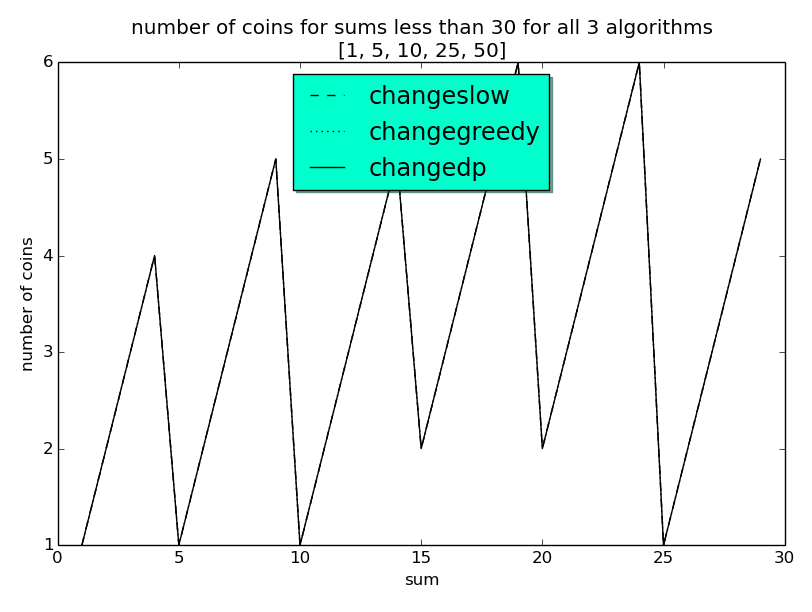
\includegraphics[width=\textwidth,height=\textheight,keepaspectratio]{q4_chart1.png}
\caption{Changeslow Algorithm}
\end{figure}
\\
\autoref{q4_chart1b.png}
\begin{figure}
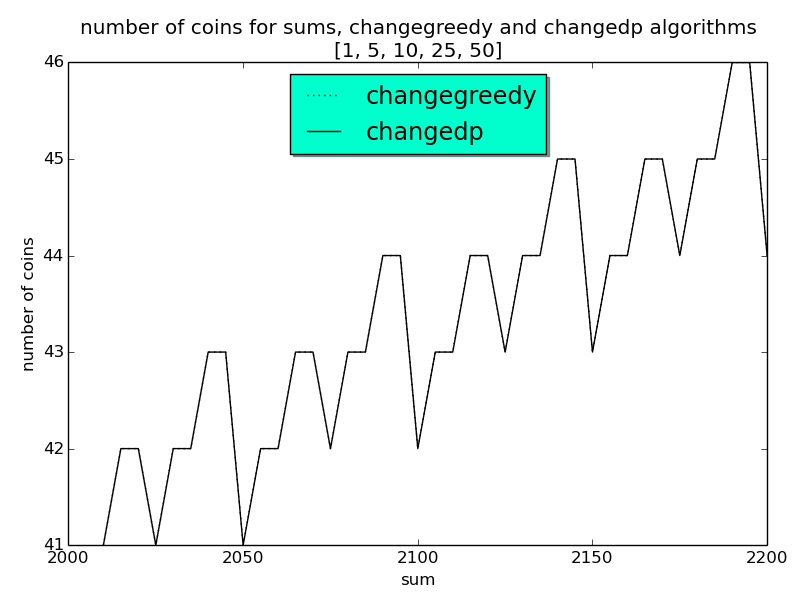
\includegraphics[width=\textwidth,height=\textheight,keepaspectratio]{q4_chart1b.png}
\caption{Changeslow Algorithm}
\end{figure}


\subsection{Suppose $V_1$ = [1, 2, 6, 12, 24, 48, 60] and $V_2$ = [1, 6, 13, 37, 150]. For each integer value of A in [2000, 2001, 2002, ..., 2200] determine the number of coins that changegreedy and changedp requires. If your algorithms run too fast try [10,000, 10,001, 10,003, ..., 10,100]. You can attempt to run changeslow however if it takes too long you can select smaller values of A and also run all three algorithms on the values. Plot the number of coins as a function of A for each algorithm. How do the approaches compare?}

\autoref{q5_chart1.png}
\begin{figure}
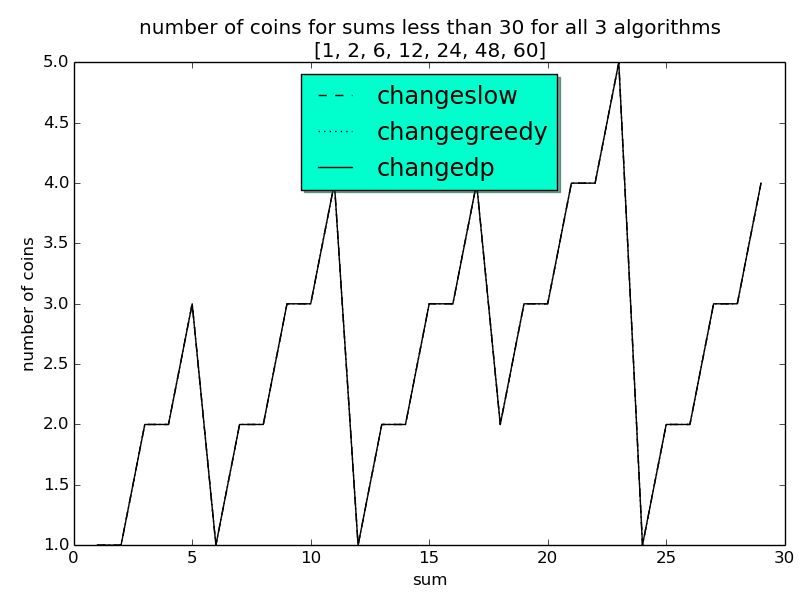
\includegraphics[width=\textwidth,height=\textheight,keepaspectratio]{q5_chart1.png}[h!]
\caption{Greedy Algorithm}
\end{figure}

\autoref{q5_chart1b.png}
\begin{figure}
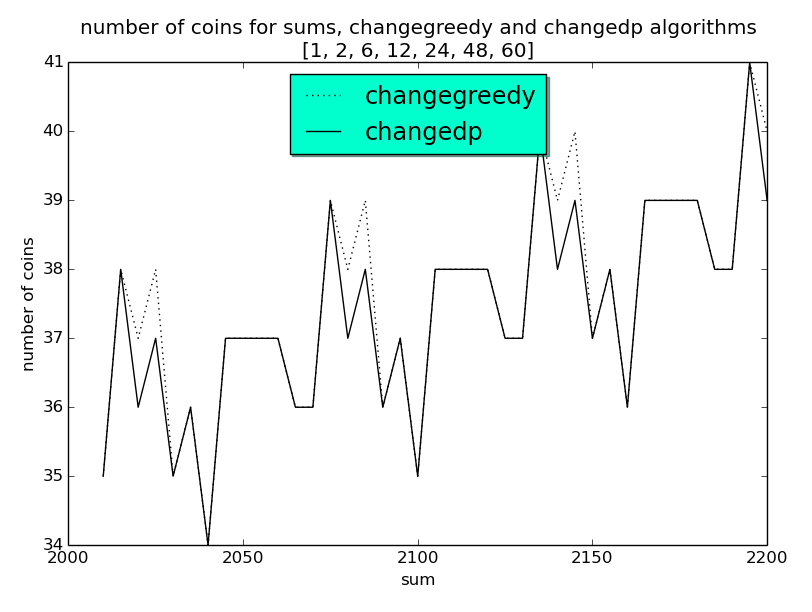
\includegraphics[width=\textwidth,height=\textheight,keepaspectratio]{q5_chart1b.png}[h!]
\caption{Greedy Algorithm}
\end{figure}

\autoref{q5_chart2.png}
\begin{figure}
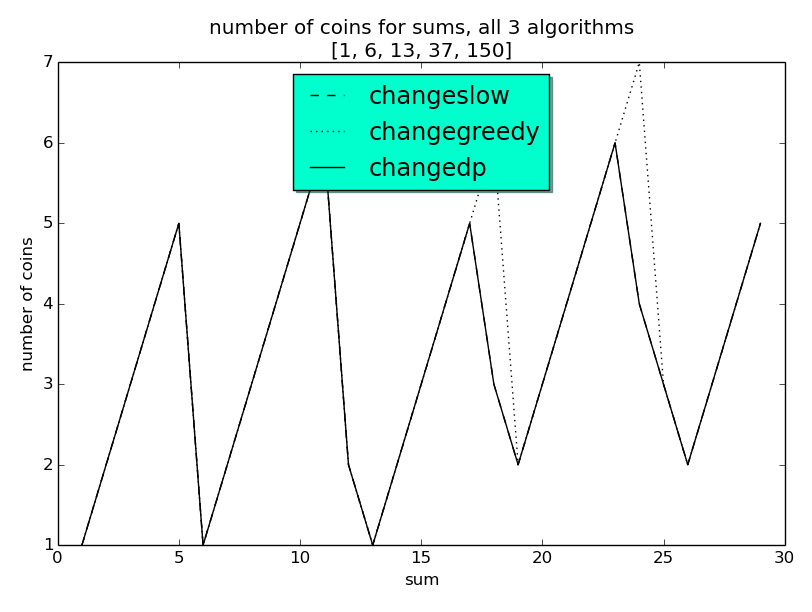
\includegraphics[width=\textwidth,height=\textheight,keepaspectratio]{q5_chart2.png}[h!]
\caption{Greedy Algorithm}
\end{figure}

\autoref{q5_chart2b.png}
\begin{figure}
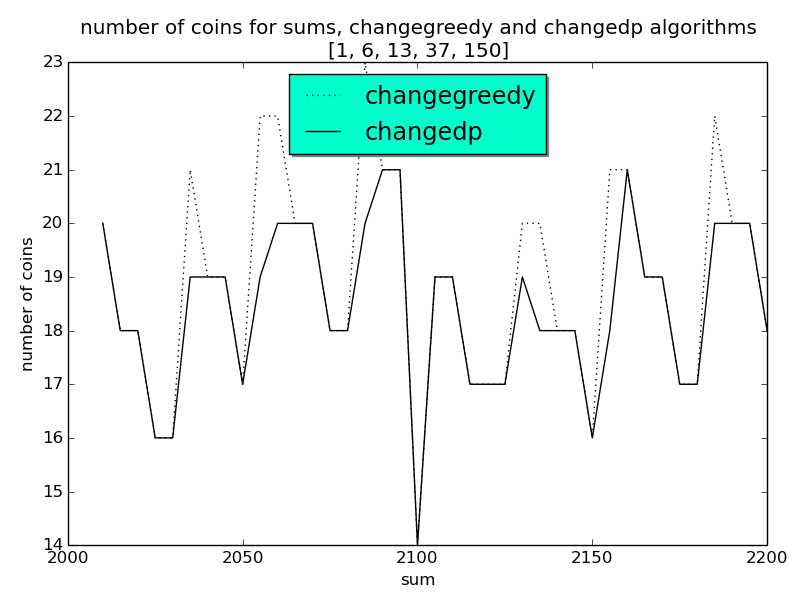
\includegraphics[width=\textwidth,height=\textheight,keepaspectratio]{q5_chart2b.png}[h!]
\caption{Greedy Algorithm}
\end{figure}

\subsection{Suppose V = [1, 2, 4, 6, 8, 10, 12, ..., 30]. For each integer value of A in [2000, 2001, 2002, ..., 2200] determine the number of coins that changegreedy and changedp requires. You can attempt to run changeslow however if it takes too long you can select smaller values of A and also run all three algorithms on the values. Plot the number of coins as a function of A for each algorithm.}

\autoref{q6_chart1.png}
\begin{figure}
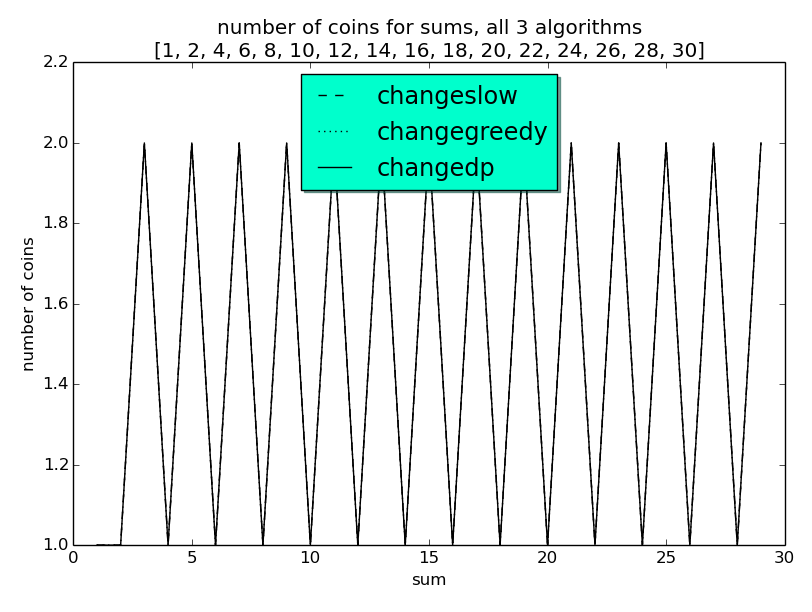
\includegraphics[width=\textwidth,height=\textheight,keepaspectratio]{q6_chart1.png}[h!]
\caption{Dynamic Programming}
\end{figure}

\autoref{q6_chart1b.png}
\begin{figure}
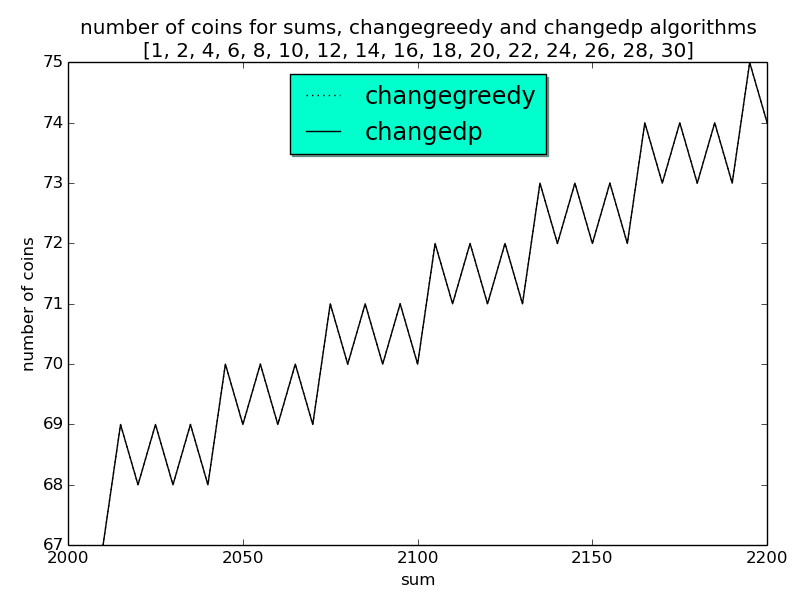
\includegraphics[width=\textwidth,height=\textheight,keepaspectratio]{q6_chart1b.png}[h!]
\caption{Dynamic Programming}
\end{figure}


\subsection{For the above situations, determine (experimentally) the running times of the algorithms by fitting trend lines to the data or analyzing the log-log plot. Graph the running time as a function of A. Compare the running times of the different algorithms.}


\subsection{Use the data from questions 4-6 and any new data you have generated. Plot running times as a function of number of denominations (i.e. V=[1, 10, 25, 50] has four different denominations so n=4). Does the size of n influence the running times of any of the algorithms?}


\subsection{Suppose you are living in a country where coins have values that are powers of p, $V = [p^0 , p^1 , p^2 , ��� , p^n]$. How do you think the dynamic programming and greedy approaches would compare? Explain}


\newpage{}
\section{Appendices}
\subsection{Code\newline}
The main used to determine the results for Project 2. 
\lstinputlisting[language=Python]{code/main.py}

\subsection{Tests\newline}
This contains the conditions and tests for our algorithms. 
\lstinputlisting[language=Python]{code/project2_rbt.py}		

\subsection{Questions\newline}
This contains code that helps to answer the questions above. 
\lstinputlisting[language=Python]{code/questions.py}	

\end{document}  